\subsubsection*{Le matin :}

Les résultats du calcul du weekend ont été récupérés.
Voici le resultat de l'apprentissage:
\begin{figure}[H]
    \center
    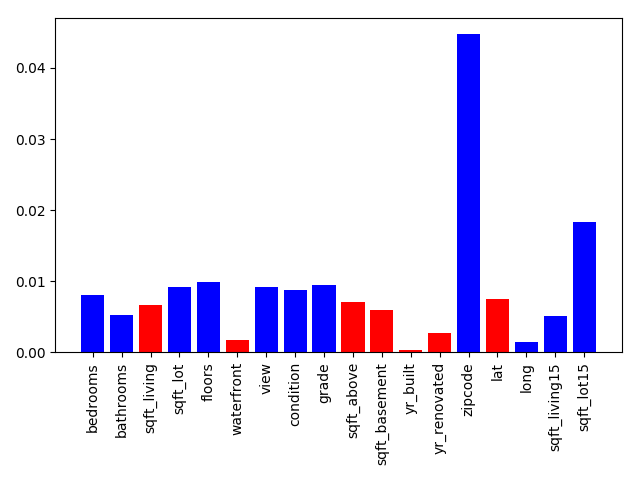
\includegraphics[height=\petit]{sources/data/Obj2/real/graphs/default_10000_1.png}
    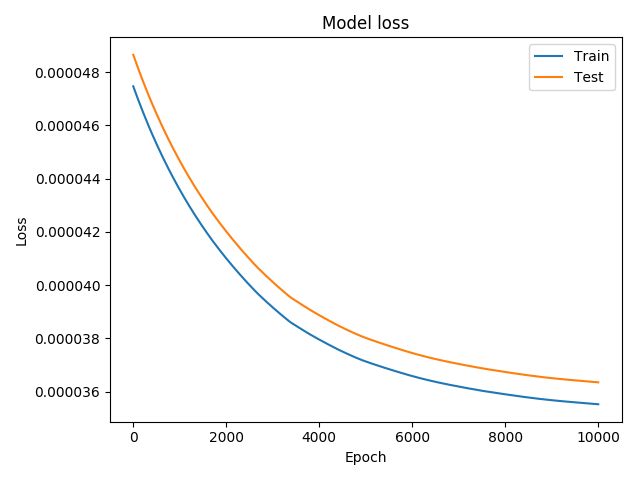
\includegraphics[height=\petit]{sources/data/Obj2/real/graphs/default_10000_1_learn.png}
	\caption{Apprentissage sur les données réelles}
	\label{def_10000_1}
\end{figure}


Comme ont peut le voir ici,
il n'y a pas d'ecarts types ce qui est très mauvais,
la matiné a alors été passée a recoder une fonction pour afficher ces ecarts types, en voici les résultats:
\begin{figure}[H]
    \center
    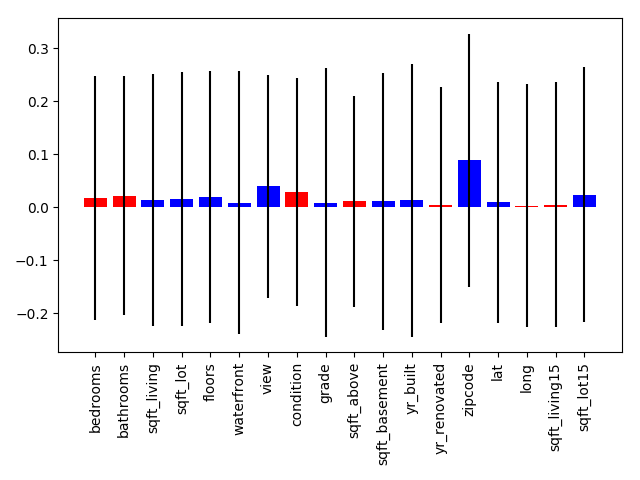
\includegraphics[height=\petit]{sources/data/Obj2/real/graphs/default_100_100.png}
    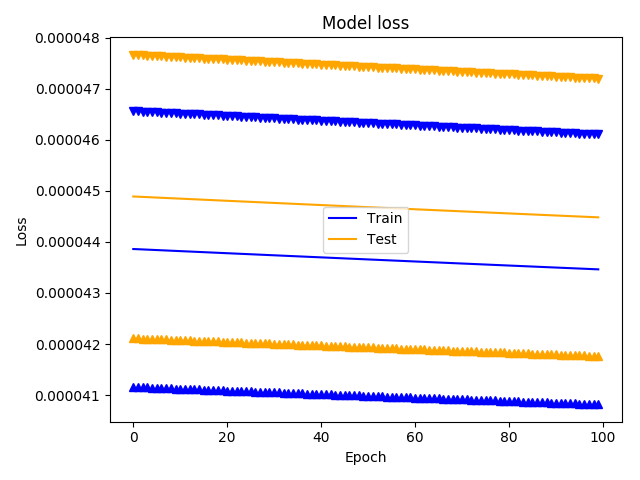
\includegraphics[height=\petit]{sources/data/Obj2/real/graphs/default_100_100_learn.png}
	\caption{Apprentissage sur les données réelles}
	\label{def_100_100}
\end{figure}
On peut voir que l'apprentissage est totalement cahotique.

\subsubsection*{L'après midi :}
Pour essayer de remetre de l'ordre dans ce chaos,
j'ai décidé de retier les parametres qui me paraissent peu significatifs.
Le parametres sont les suivants:
\begin{itemize}
    \item[view :] Nombre de fois que la maison à été visitée avant son achat.
    \item[Parametres géographiques :]
        Même si ils ont une importance (réputation du cartier),
        il infulencent déja d'autres parametres.
    \item[Année de construction :] fusionné avec les derniers travaux.
\end{itemize}

Les résultats sont les suivants:
\begin{figure}[H]
    \center
    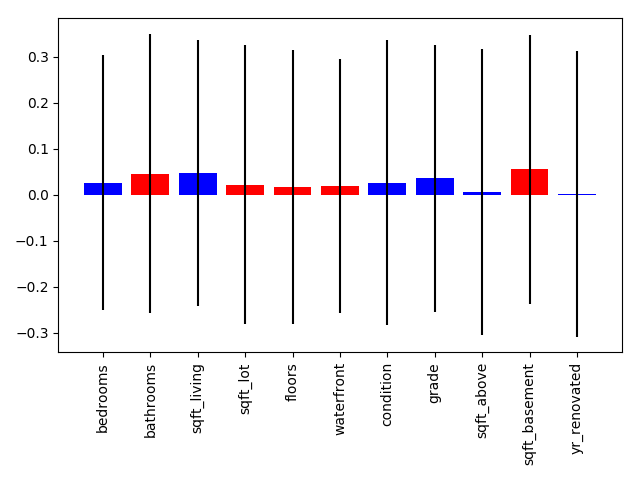
\includegraphics[height=\petit]{sources/data/Obj2/real/graphs/remove1_100_100.png}
    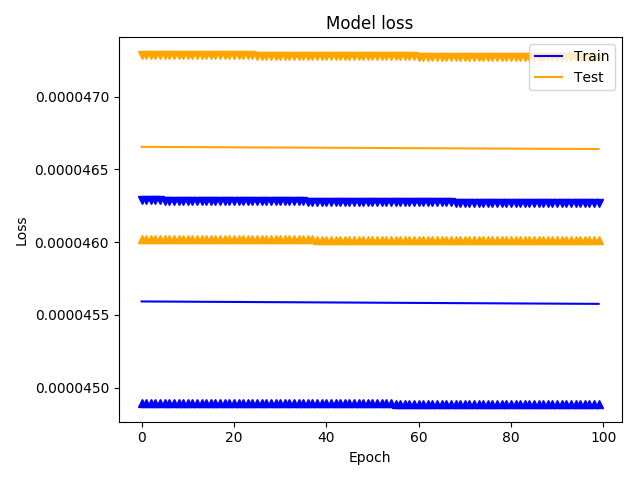
\includegraphics[height=\petit]{sources/data/Obj2/real/graphs/remove1_100_100_learn.png}
	\caption{Apprentissage sur les données réelles}
	\label{r1_100_100}
\end{figure}
On peut voir que de meme que dans la Fig.\ref{def_100_100}, les résultats ne sont pas probants.
Ces variations sont surement dues au grand nombre de paramètres,
la fin de l'après midi a donc été passée à tester le lien entre diferents parametres et le prix via de nombreuses regressions.
